% % % % % % % % % % % % 
% % %  N O T E S % % %
% - before compiling the final version, uncomment the correct `documentclass` line
% - requires LuaLaTex compiler (for the slide 'SHAP values -- working example')
% - due to compilation time, some slides are included via `input` command and need to be uncommented before compiling the final version
% % % % % % % % % % % % 


%% Semplice beamer conforme al powerpoint ufficiale
%% dal sito di Ca' Foscari. Si basa sul tema "default"
%% mandate Modifiche e migliorie! Guido.Caldarelli@unive.it 
% Elenco Contributori 
% Guido Caldarelli, Matteo Brilli 

%\documentclass{beamer}
% decide below the aspect ratio between 16:9 and 4:3
% \documentclass[aspectratio=43]{beamer}
% \documentclass[aspectratio=169]{beamer}       % UNCOMMENT FOR UNCOVER TO WORK
\documentclass[aspectratio=169,handout]{beamer} % DEACTIVATES UNCOVER, FOR FINAL VERSION COMMENT THIS LINE OUT AND UNCOMMENT THE LINE ABOVE

\usepackage[utf8]{inputenc}

% Questo tema commentato di sotto produce un beamer più tradizionale 
%\usetheme[secheader]{Boadilla}


%%%-----------------------------------------------------------%
%% Cambia colori da thema default
%% Questi sono i due colori ufficiali rosso e grigio
\definecolor {cfred}{rgb}{0.709,0.196,0.329} 	%{ 181 ,50 ,84}
\definecolor {cfgrey}{rgb}{0.537,0.537,0.537} 	%{ 137,137,137}
\definecolor {cflink}{rgb}{0.615,0.615,0.607} 	%{157,157,155}

\setbeamercolor{palette primary}{bg=cfred,fg=white}
\setbeamercolor{palette secondary}{bg=cfred,fg=white}
\setbeamercolor{palette tertiary}{bg=cfred,fg=white}
\setbeamercolor{palette quaternary}{bg=cfred,fg=white}
\setbeamercolor{structure}{fg=cfred}		 % itemize, enumerate, etc
\setbeamercolor{section in toc}{fg=cfred} 		 % TOC sections
% Override palette coloring with secondary
\setbeamercolor{subsection in head/foot}{bg=cfgrey,fg=white}
%%%------------------------------------------------------------

%% Definisce il blocco con riquadro che non è presente nel tema default (commentare se si usano altri temi)
\setbeamercolor{uppercolor}{fg=white,bg=cfred}%
\setbeamercolor{lowercolor}{fg=black,bg=white}%
\def \bblock{\begin{beamerboxesrounded}[upper=uppercolor,lower=lowercolor,shadow=true]}
\def \eblock{\end{beamerboxesrounded}}
%%-----------------------------------------------------------

%% Intestazione ripetuta per ogni slide
\addtobeamertemplate{headline}{%
\vspace{0.25cm} \ \ 
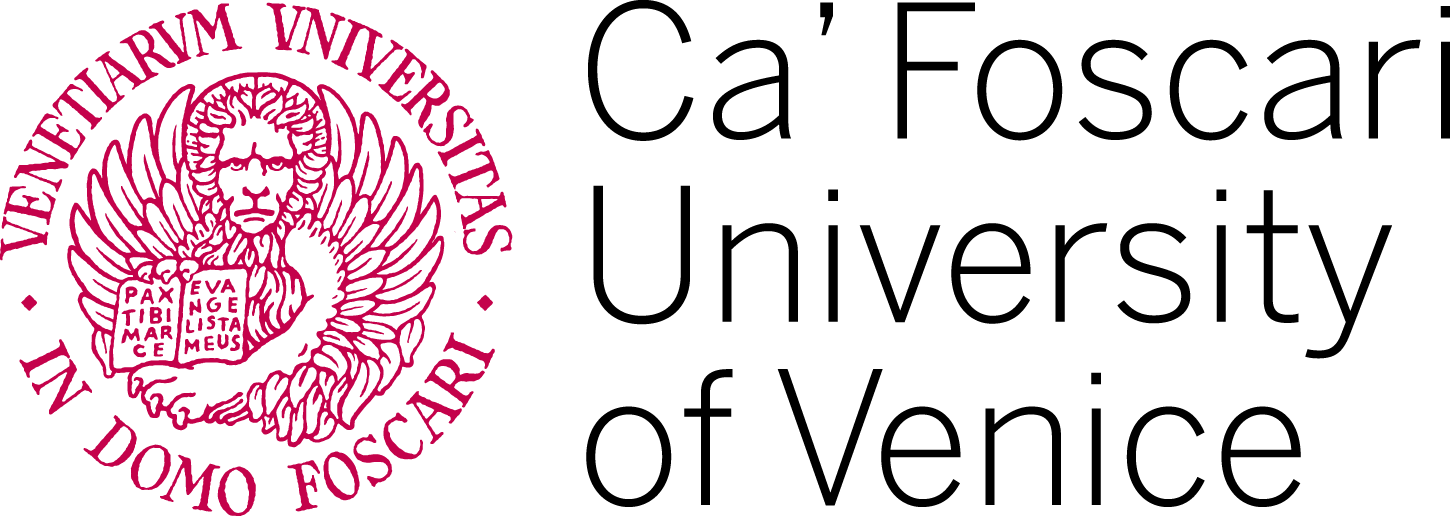
\includegraphics[height=1.0cm]{logobeamEN.png} 	% sostituire con logobeamIT.png per italiano
\hspace{0.641\textwidth}{\color{cflink} {\small www.unive.it}} %per 16:9
%\hspace{0.551\textwidth}{\color{cflink} {\small www.unive.it}} %per 4::3

\vspace{0.25cm}
{\color{cfred} \hrule \hrule  }
\textbf{}
}{}
%%-------------------------------------------------------------


%------------------------------------------------------------
%The next block of commands puts the table of contents at the 
%beginning of each section and highlights the current section:

\AtBeginSection[]
{
  \begin{frame}
    \frametitle{Table of Contents}
    \tableofcontents[currentsection]
  \end{frame}
}
%------------------------------------------------------------

% poniższy złoty kawałek kodu przy rozpoczęciu każdej nowej sekcji robi slajd pokazujący, gdzie jesteśmy
% \AtBeginSection[]{
%   \begin{frame}{Outline}
%   \setbeamertemplate{section in toc}[sections numbered]
%   \tableofcontents[currentsection, hideothersubsections]
%   \end{frame} 
% }

% \AtBeginSubsection[]{
%   \begin{frame}{Outline}
%   \setbeamertemplate{section in toc}[sections numbered]
%   \tableofcontents[currentsection, currentsubsection]
%   \end{frame} 
% }


% grey text
\definecolor{lightgray}{RGB}{211,211,211}
\newcommand\gray[1]{{\color{lightgray}{#1}}}

% compatibility colours
\definecolor{cinnamon}{RGB}{205,92,92}

% emoji for SHAP working example
\usepackage{fontspec}  % emoji
\newfontfamily{\NotoEmoji} {NotoColorEmoji.ttf}[Renderer=Harfbuzz]
% % % % % % % % % % % % % % % % % % %
%   THE COMPILER MUST BE LUALATEX   %
% % % % % % % % % % % % % % % % % % %


% TITLE PAGE
\title[About Beamer] %optional
{About the Beamer class for Ca'Foscari researchers}\subtitle{A short story}

\author[Newton, Darwin] % (optional)
{I.~Newton\inst{1} \and C.~Darwin\inst{2}}

\institute[VFU] % (optional)
{
  \inst{1}%
  Department of Molecular Sciences and Nanosystems\\
  Ca' Foscari University, Via Torino 155, 30170 Venezia Mestre, Italy
  \and
  \inst{2}%
  European Centre for Living Technologies (ECLT)\\
 Ca' Bottacin, 3911 Dorsoduro Calle Crosera, 30123 Venice, Italy
 }

\date[VLC 2014] % (optional)
{Very Large Conference, April 2020}

\setbeamertemplate{frametitle}[default][right, rightskip=.5cm] {}
\addtobeamertemplate{frametitle}{\vspace*{-1.4cm}}{}
%End of title page configuration block
%------------------------------------------------------------

\setbeameroption{show notes}  % uncomment to see the notes
\setbeamertemplate{note page}[plain]  % simpler style for notes

\usepackage{todonotes}
\newcommand{\AW}[1]{\todo[inline, backgroundcolor=teal!20, author=AW]{#1}}

\begin{document}

%The next statement creates the title page.
\frame{\titlepage}
%---------------------------------------------------------
%This block of code is for the table of contents after
%the title page
\begin{frame}
\frametitle{Table of Contents}
\tableofcontents
\end{frame}
%---------------------------------------------------------



% % % % % % % % % % % %
%   U N C O M M E N T %
% % %  I N T R O  % % %
% 
\section{Introduction}

\begin{frame}{Motivation}
    slide with dogs (it takes forever to compile)

    % % % %
    \note{
        \tiny
        \begin{enumerate}
            \item we start with a story to attract attention
            \item story: AI is present in more and more of areas of our life $\rightarrow$ it is extremely important to ensure that the models are safe/perform well
            \item motivation: model evaluation is not enough -- models can utilise biases present in the data: use wrong features and still get a high performance
            \item therefore, we want to ensure that \textbf{models make good predictions based on the right features}
            \item explainability allows to do just that
            \item let's see an example
            \item task: telling apart huskies from wolves based on pictures
            \item 1st step: build training data and use it to train the model
            \item 2nd step: the model is trained, it has a good accuracy, we present it with a new picture, the model makes a mistake
            \item 3rd step: we explain the prediction to understand what happened
            \item conclusion: the model looked at the background not at the animal in the picture
            \item why it happened: back to our training data: all huskies are on green grass, all wolves are on white snow, telling apart huskies from wolves is difficult, but telling apart green from white is something convolutional networks are good at and it's easy for them $\rightarrow$ the model took a shortcut/used the bias present in the data
            \item the bias was present in both the train and the validation set which is why the model had a good performance
            \item the test set doesn't have this bias, so we are surprised to see our high performing model make lots of mistakes
            \item explainability can reveal why these mistakes happen
            \item actually: if we used explainability during the validation stage, we would discover that our models makes predictions based on incorrect features and we would not deploy it
        \end{enumerate}
    }
\end{frame}


\begin{frame}{EXAI intro}
    \begin{itemize}
        \item what is explainability
        \item how it is different from interpretability
        \item why is it important (generalise from the story)
        \item Complex models are inherently complex -- if we want to explain the whole model, the explanation itself would be complex. But we can explain a single prediction because it involves only a small piece of that complexity.
    \end{itemize}
\end{frame}


\begin{frame}{Explainability definition}
    put some definition here: black box, ... some images
\end{frame}

\begin{frame}{Explainability vs interpretability}
    image
    % % % %
    \note{
    \begin{enumerate}
        \item explainability - black-box
        \item interpretability - white-box
        \item high-stake decisions (trials, loans) -- better use interpretable models
        \item but building interpretable models is usually more difficult than building any models (out of the box XGBoost/neural network will usually have a decent performance but it's not interpretable)
        \item so we can compromise if the decisions are not high-stake: use black-box models and explain them!
    \end{enumerate}
    }    
\end{frame}

\begin{frame}{Explainability vs AI}
    image
    \AW{NOT SURE IF WE WANT THIS SLIDE?}
    \AW{that's the picture that shows that the focus in AI is on what the prediction is, while the focus in AI is on the model (why is the prediction such and not other)}
\end{frame}

\begin{frame}{Tasks}
    task that can be solved with explainability (model debugging, model trust, scientific discovery)
    \AW{not sure if we want this here? maybe we only want it in jupyter notebooks? on the other hand it would give some context...}
\end{frame}


\begin{frame}{math concepts intro}
    \AW{probably will need to move somewhere else or introduce them when needed}    
\end{frame}



\section{Working example}
\begin{frame}{working example}
    \begin{itemize}
        \item life-situation example
        \item linear regression
        \item AND op?
    \end{itemize}
\end{frame}

\begin{frame}{Example 1 -- AND}
    What is the relative importance of these features?

    A = 1, B = 1

    And in this case?

    A = 0, B = 1

    \note{
    \begin{itemize}
        \item Let's see how a simple explanation can look like.
        \item A common way of explaining predictions is to assign a single scalar value to each feature.
        \item Let's try to provide explanations for the math AND operator.
        \item We will try to answer which features are important for predicting the outcome.
        \item In the first example, both features are important -- we need to know both of them to predict the outcome. They also don't differ so we can give both of them 50\% of responsibility for the outcome.
        \item In the second example, knowing only the value of A is enough, we can attribute the entire responsibility for the outcome to this feature, so the responsibility/importance values will be 100\% and 0\%
    \end{itemize}
    }
\end{frame}

\begin{frame}{Example 2 -- linear regression}
    \AW{agni.wojt: diabetes-example.ipynb}
    $$y = X \cdot w + b$$

    \note{
    \begin{itemize}
        \item introduce oznaczenia
        \item ask how they would explain linear regression model's predictions
        \item show difference between rank based on features and rank based on features * coefficients
        \item introduce a concept: importance scores of all features sum to the prediction
        \item show decision plot
    \end{itemize}
    }
\end{frame}

\begin{frame}{Example 3 - different explanations}
    \AW{how explanations can look like -- I think this slide would be helpful?}
\end{frame}


% % % % % % % % % % % %


\section{SHAP}

\begin{frame}{SHAP}
    \begin{itemize}
        \item additive feature attribution method
        \item explains how to get from the base prediction (mean prediction of the model) to the actual prediction
        \item suitable for tabular data \gray{(e.g. fingerprints)}
        \item both classification and regression
        \item model-agnostic \gray{-- works with any model}
        \item provides local explanations \gray{-- explains predictions (not the entire model)}
        \item perturbation-based \gray{-- calculates explanations by perturbing, i.e. introducing small changes into, the input instance}
        \item based on Shapley values from game theory -- nice mathematical guarantees
        \item can be rather slow but there exist model-specific fast alternatives
        \item prone to unrealistic data instances
    \end{itemize}

    \AW{image with an exemplary explanation}
    \AW{decision plot with the same explanation}

    \note{
    \footnotesize
    \begin{itemize}
        \item \textbf{introduce term: additive feature attribution model} $\rightarrow$ it's like our regression example
        \item which is why it's suitable for tabular data (just as linear regression)
        \item \textbf{introduce term: model-agnostic} -- this means that it works with any model, be it linear regression, decision trees, support vector machines...
        \item \textbf{introduce term: local explanation}
        \AW{\tiny warto gdzieś na slajdzie dorzucić: Complex models are inherently complex -- if we want to explain the whole model, the explanation itself would be complex. But we can explain a single prediction because it involves only a small piece of that complexity.}
        \item \textbf{introduce term: perturbation-based}
        \item \textbf{game theory} -- deals with mathematically proving if a player has a winning strategy, e.g. white does not have a winning strategy -- there is no single strategy that ALWAYS leads to winning no matter what black does; on the other hand, in tic-tac-toe the starting player has a winning strategy
        \item we will introduce \textbf{Shapley values} and the resulting mathematical guarantees in a minute
        \item we will focus on kernelSHAP which is the (slow) model-agnostic algorithm, we will use TreeSHAP, which is optimised for tree-based models, during the practical part (==possibly== preferentially)
        \item \textbf{unrealistic data instances} are due to SHAP being a permutation-based method, \#~out-of-distribution
    \end{itemize}

    }
\end{frame}


% % % % % % % % % % % %
%   U N C O M M E N T %
% S H A P L E Y   V A L U E S %
% 
\begin{frame}{Shapley values}
    \begin{center}
    \begin{minipage}{0.4\textwidth}
    \begin{center}
 	   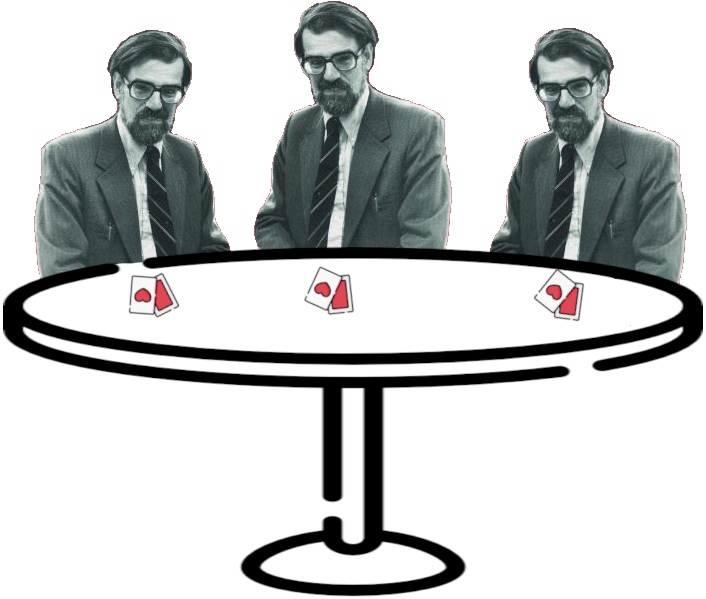
\includegraphics[width=0.9\linewidth]{fig/shapley-game.png}
    \end{center}
    \end{minipage}
    \begin{minipage}{0.55\textwidth}
    \begin{itemize}
        \item multi-player coalition game \gray{-- the players work together to gain the biggest reward they can}
        \item the reward is then divided between the players
    \end{itemize}
    \end{minipage}    
    \end{center}
    
    \textbf{Problem:} How to split the total payout (reward) between the players in \textbf{a fair way}, i.e. taking into consideration their contribution?

    \vspace{0.05in}  % THAT'S UGLY
    Shapley showed that there exists \textbf{a unique solution} to this problem.
    
    \note{
    \begin{itemize}
        \item oh, that's Shapley in the picture
        \item \textbf{multi-player coalition game} -- the players work together to gain the biggest reward possible
        \item the reward must be shared between the players -- so it's an additive feature attribution method (or additive player contribution distribution)
        \item how to do this in \textbf{a fair way}?
        \item Well, first we need to define mathematically, what does it mean 'a fair way'.
        \item And, BTW, Shapley has shown that there is \textbf{a unique way} of doing this, i.e. \textbf{a unique solution}
    \end{itemize}
    }
\end{frame}


\begin{frame}{The fairness properties}
    \begin{block}{\textbf{Efficiency}}
    The entire reward must be split.
     % The feature contributions must add up to the difference of the prediction for $x$ and the~\textbf<2>{average} prediction.
    
    % $\sum\nolimits_{j=1}^p\phi_j=\hat{f}(x)-E_X(\hat{f}(X))$
    \end{block}
    
    % \uncover<2->{
    \begin{block}{\textbf{Symmetry}}
    If two players contributed equally then their payout should be the same.
    
    % The contributions of two feature values $j$ and $k$ should be the same if they contribute equally to all possible coalitions.
    
    % If $val(S\cup\{x_j\})=val(S\cup\{x_k\})$
    % for all
    % $S\subseteq\{x_{1},\ldots,x_{p}\}\setminus\{x_j,x_k\}$
    % then
    % $\phi_j=\phi_{k}$
    \end{block}
    % }

    % \uncover<3->{
    \begin{block}{\textbf{Dummy}}
    A player who has no impact on the reward value gets no reward.
    
    % A feature $j$ that does not change the predicted value -- regardless of which coalition of feature values it is added to -- should have a Shapley value of $0$.    
    % If $val(S\cup\{x_j\})=val(S)$
    % for all
    % $S\subseteq\{x_{1},\ldots,x_{p}\}$
    % then
    % $\phi_j=0$
    \end{block}
    % }
    
    % \uncover<4->{
    \begin{block}{\textbf{Additivity}}
    If players play one game after another then calculating their rewards after each game should give the same result as calculating their total rewards once, after the last game.
    
    % For a game with combined payouts $val+val^+$ the respective Shapley values are as follows:
    % $\phi_j+\phi_j^{+}$
    \end{block}
    % }

    \note{
    \AW{I'm rewritting these properties to be less mathematical. We'll get lost in the details later. And this is when we'll deal with that and see how much simplification is allowed.}
    \AW{the cat working example already requires the notion of ALL coalitions}
    \begin{itemize}
        \item Once these properties are properly, mathematically defined, it turns out (i.e. Shapley has shown) that there is a unique solution.
        \item This means that splitting the reward with any other way than Shapley values breaks at least one of these properties, and thus, is unfair.
    \end{itemize}
    }
    
\end{frame}



\begin{frame}{The unique solution}
     \textbf{Definition:} The Shapley value is the average marginal contribution of a feature value across all possible coalitions.
    
    % The Shapley value of a feature value is its contribution to the payout, weighted and summed over all possible feature value combinations:
    
    % \begin{equation*}
    % \phi_j(val)=\sum_{\color<2->{cinnamon}{S\subseteq\{x_{1},\ldots,x_{p}\}\setminus\{x_j\}}} \frac{|S|!\left(p-|S|-1\right)!}{p!}\left(val\left(S\cup\{x_j\}\right)-val(S)\right)    
    % \end{equation*}

    
    % \begin{equation*}
    % \footnotesize
    % \phi_j(val)=
    % {\sum_{
    % \underbrace{S\subseteq\{x_{1},\ldots,x_{p}\}}_{\substack{\uparrow \\ \text{all possible coalitions} \\ \text{of $p$ players}}}
    % \underbrace{\setminus\{x_j\}}_{\substack{\uparrow \\ \text{without} \\ \text{player $j$}}}
    % }  % end \sum
    % }  % end \sum description 
    % \frac{
    % \overset{\substack{\text{no. of sequences}\\ \text{of players from $S$}\\\downarrow}}{|S|!}
    %  \overset{\substack{\text{no. of sequences of}\\ \text{the remaining players}\\\downarrow}}{\left(p-|S|-1\right)!}}
    % {\underset{\substack{\uparrow \\ \text{no. of sequences} \\ \text{of all players}}}{p!}}
    % \left(
    % \underbrace{val\left(S\cup\{j\}\right)}_{\substack{\uparrow \\ \text{reward with player $j$ present} \\ \text{player $j$}}}
    % -
    % \underbrace{val(S)}_{\substack{\uparrow \\ \text{ reward without} \\ \text{player $j$}}}\right)
    % \end{equation*}

    \begin{equation*}
    \phi_j(val)=
    {\sum_{
    \underbrace{S\subseteq\{x_{1},\ldots,x_{p}\}}_{\substack{\uparrow \\ \text{all possible coalitions} \\ \text{of at most $p$ players}}}
    \underbrace{\setminus\{x_j\}}_{\substack{\uparrow \\ \text{without} \\ \text{player $j$}}}
    }  % end \sum
    }  % end \sum description 
    \underbrace{\frac{|S|!(p-|S|-1)!}{p!}}_{\substack{\uparrow \\ \text{weighting factor}}}
    \underbrace{
    (
    \overbrace{val(S\cup\{j\})}^{\substack{\text{reward with} \\ \text{player $j$ present} \\ \downarrow }} 
    - \overbrace{val(S)}^{\substack{\text{reward without} \\ \text{player $j$} \\ \downarrow }} )
    }_{\substack{\uparrow \\ \text{$j$'s contribution for coalition $S$} }}
    \end{equation*}

    \note{
    \begin{itemize}
        \item read the definition
        \item \textbf{explain: marginal contribution} -- contribution of the player regardless of other players
        % (wiki) In probability theory and statistics, the marginal distribution of a subset of a collection of random variables is the probability distribution of the variables contained in the subset. It gives the probabilities of various values of the variables in the subset without reference to the values of the other variables.
        % so we want contribution of the player regardless of other players
        \item \textbf{explain: coalition} -- a subset of players
        % \item \textbf{note: across all possible coalitions} -- so over all sequences
        % \item note: average -- and we'll have to do some averaging
        \item warn that we will now express it mathematically
        \item go through the equation step by step
        \item \textbf{the contribution of player $j$} is the difference between the reward with him playing and the reward without him playing
        
        \item OK, on the following slides we'll discuss the weighting factor
    \end{itemize}
    }

\end{frame}

\begin{frame}{Order matters}
    \footnotesize
    Order matters when the function is nonlinear or the variables are not independent.

    \textbf{Nonlinearity:} let's go back to our AND example. A = 0, B = 1
    \begin{itemize}
        \item if we learn about A first, then it gets the entire contribution -- we already know what would be the answer -- and so B will get 0 contribution
        \item but if we learn first about B, then we still don't know what the answer would be -- thus A and B will get equal contribution
    \end{itemize}

    \textbf{Dependent variables:}
    \begin{itemize}
        \item we have four variables: A, B, C, D; B = C + D (so B and C, and B and D are dependent)
        \item we predict the sum of all the variables
        \item if we learn about the variables in order: A, B, C, D; then C and D have no contribution -- once we know A and B, we know that the sum is A + 2B
        \item if we learn about the variables in order: A, C, D, B, then C and D have nonzero contribution, but B has zero contribution -- once we learn about A, C, D, we know that the sum is A + 2 * (C + D)
    \end{itemize}

    When calculating Shapley values, all possible orderings are considered and an average contribution is calculated.

    \note{
    Which ordering to choose when calculating contribution? The answer is to consider all of them.
    }
\end{frame}

\begin{frame}{Weighting factor for a coalition of players}
    When calculating $j$'s contribution for some coalition $S$ we need to know how many sequences correspond to this situation:

    \begin{itemize}
        \item $|S|$ players can be ordered in $|S|!$ sequences
        \item the remaining players can be ordered in $(p - |S| - 1)!$ sequences
        \item coalition $S$ corresponds to $|S|!(p - |S| - 1)!$ sequences
    \end{itemize}

    There are $p!$ sequences of $p$ players, so each sequence has weight $\frac{1}{p!}$

    Therefore, the weight for $j$'s contribution to coalition $S$ is:
    $$\frac{|S|!(p - |S| - 1)!}{p!}$$

    % Molnar: Intuitive understanding of Shapley values
    % The feature values enter a room in random order. All feature values in the room participate in the game (= contribute to the prediction). The Shapley value of a feature value is the average change in the prediction that the coalition already in the room receives when the feature value joins them.

    \note{
    OK, so order matters. But we would like to use subsets not sequences but subsets are unordered. So... we need to employ some combinatorics!
    }
\end{frame}



% % % % % % % % % % % %


\begin{frame}{Shapley values -- plan}
\footnotesize
\begin{itemize}
        % \item one-slide overview (how it works in one slide)
        % \item why is it good and what is it good for (tabular data, reg+cls., etc.)
        % \begin{itemize}
        %     \tiny
        %     \item black box (any function will work, but knowing the model's family the computations can be sped up)
        %     \item local but can give some global insight (explains predictions, but explaining the whole dataset and doing clever statistics gives insight into the whole model)
        %     \item fast computation
        %     \item attractive theoretical guarantees arising from game theory
        %     \item excellent performance on explainability metrics
        %     \item helps to select important features
        %     \item is consistent with human intuition
        %     \item Like many other permutation-based interpretation methods, the Shapley value method suffers from inclusion of unrealistic data instances when features are correlated.
        % \end{itemize}
        % \item \textbf{Additive feature attribution} models are one family of explainability models. They try to attach a single scalar value to each feature, this value reflects the credit attributed to this feature. $\rightarrow$ \textbf{(working example) linear regression} (1. how to explain it; 2. how it is similar to additive feature attribution models); how did we get from the base prediction (ex. a mean prediction for the entire training set) to the actual prediction? (+ image of decision graph)
        % \item in depth math
        % \item summary
        \item kernelSHAP takes long to calculate, there are model-specific approaches (e.g. TreeSHAP) that are faster. We'll focus on kernelSHAP.
    \end{itemize}

% \begin{itemize}
    % \item its a game
    % \item arises from game theory (probably should explain in two sentences what it is: game problems, winning strategy, kolko i krzyzyk, chess)
    % \item problem formulation (how to split the reward in a fair way) + intuition: it sums $\rightarrow$ so it's linear regression
    % \item the properties $\rightarrow$ unique solution
    % \item definition: The Shapley value is the average marginal contribution of a feature value across all possible coalitions.
% \end{itemize}

The Shapley value of a feature value is its contribution to the payout, weighted and summed over all possible feature value combinations:

The interpretation of the Shapley value for feature value $j$ is: the value of the $j$-th feature contributed $\phi_j$ to the prediction of this particular instance compared to the average prediction for the dataset.

\textbf{compared to the average prediction for the dataset} -- This covers situations in which players get some starting reward when they start playing, so if players do not contribute are all for the entire game, they still get the starting reward. Shapley values tell us how to split the rest of the reward. (And yes! They can be negative! So a reward for a bad player might in fact be a punishment -- the player has to pay!)

\textbf{Intuition:}

% The interpretation of the Shapley value for feature value $j$ is: The value of the $j$-th feature contributed $\phi_j$ to the prediction of this particular instance compared to the average prediction for the dataset.

Be careful to interpret the Shapley value correctly: The Shapley value is the average contribution of a feature value to the prediction in different coalitions. The Shapley value is NOT the difference in prediction when we would remove the feature from the model.

\end{frame}





\begin{frame}{Shapley values $\rightarrow$ SHAP values}
    \AW{image should be redone)}
    \centering
    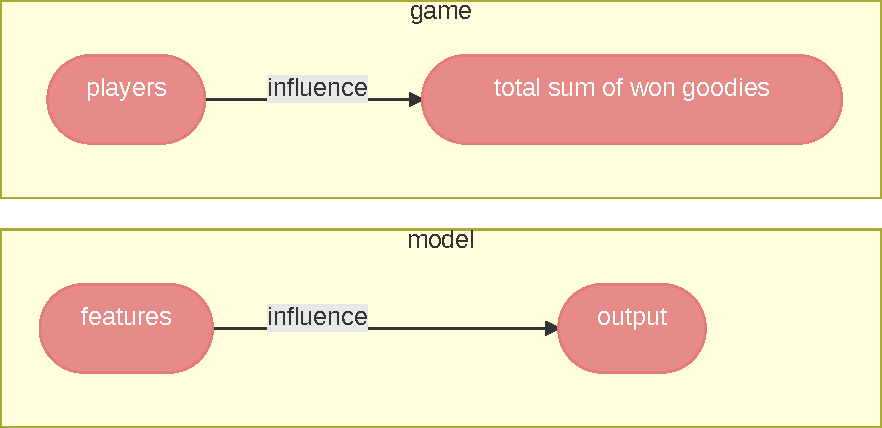
\includegraphics[width=0.7\linewidth]{fig/MLgame.pdf}

    OK, but when calculating Shapley values we could play out an imaginary scenario in which some players were not taking part in the game. In AI setup, this would correspond to not knowing values of some features. But most AI models don't accept missing features!
\end{frame}


\begin{frame}{Missing players -- missing features}
    Thus:

    \begin{center}
    SHAP values are not exactly the same as Shapley values.
    
    SHAP values are the Shapley values of \textbf{a conditional expectation function of the original model.}
    \end{center}

    Wait, what?!

    Although one cannot calculate a prediction when a feature is missing, one can pretend not to know its value. $\rightarrow$ the value of the ‘missing’ feature is replaced with any value from the dataset and prediction can be easily calculated.

    \note{
    \textbf{conditional expectation} -- we assume to know values of only some features (the features on which we condition) and calculate the expected prediction (expected, not exact, because the unknown features can take different values -- depending on these values we will get different predictions)
    }
    
\end{frame}


\begin{frame}{Intuition: conditional expectation and why order matters revisited}
    \AW{Fig. 1 from NIPS SHAP paper}

    \note{

    Fig 1. shows a single ordering. When the model is non-linear or the input features are not independent, however, the order in which features are added to the expectation matters, and the SHAP values arise from averaging the $\phi_i$ values across all possible orderings.
    }
\end{frame}


% % % % % % % % % % % %
%   U N C O M M E N T %
% this is a really nice slide, but it's already split into 12 slides
% 
\begin{frame}{SHAP values -- working example}
    \footnotesize
    \begin{minipage}{0.33\textwidth}
        Let's predict apartment price based on four features:
        
        \begin{itemize}
            \item {\NotoEmoji \symbol{"1F947}}, {\NotoEmoji \symbol{"1F948}}, {\NotoEmoji \symbol{"1F949}} -- floor
            \item {\NotoEmoji \symbol{"1F522}} -- size
            \item {\NotoEmoji \symbol{"1F333}}, {\NotoEmoji \symbol{"1FA93}} --  park nearby?
            \item {\NotoEmoji \symbol{"1F63A}}, {\NotoEmoji \symbol{"1F63F}} -- are cats allowed?
        \end{itemize}
        
        % Let's say we have a house on 2nd floor, 50m$^2$ big, with a nearby park and no cats allowed and it's value was predicted to be 300K
        \uncover<2->{\vspace{.15in}
        ({\NotoEmoji \symbol{"1F948}}, {\NotoEmoji \symbol{"1F522}}50m$^2$, {\NotoEmoji \symbol{"1F333}}, {\NotoEmoji \symbol{"1F63F}}) $\rightarrow$ 300K}
        
        \uncover<3->{\vspace{.15in}
        What is the contribution of the cat feature {\NotoEmoji \symbol{"1F63F}}?}
    \end{minipage} 
    \begin{minipage}{0.65\textwidth}
    \begin{enumerate}
        % \item<4-> Find the average prediction for all apartments: 310K.
        \item<4-> Sample a coalition of features: {\NotoEmoji \symbol{"1F522}}50m\(^2\), {\NotoEmoji \symbol{"1F333}}
        \item<5-> Sample the values for the missing features: {\NotoEmoji \symbol{"1F947}}
        \item<6-> Prediction for the new sample: {\NotoEmoji \symbol{"1F947}}, {\NotoEmoji \symbol{"1F522}}50m\(^2\), {\NotoEmoji \symbol{"1F333}}, {\NotoEmoji \symbol{"1F63F}} $\rightarrow$ 310K
        \item<7-> Replace the cat feature with a randomly drawn value: {\NotoEmoji \symbol{"1F63F}} $\rightarrow$ {\NotoEmoji \symbol{"1F63A}}
        \item<8-> Prediction for the new sample: {\NotoEmoji \symbol{"1F947}}, {\NotoEmoji \symbol{"1F522}}50m\(^2\), {\NotoEmoji \symbol{"1F333}}, {\NotoEmoji \symbol{"1F63A}} $\rightarrow$ 320K
        \item<9-> The contribution of the cat feature is: 310K - 320K = -10K
        \item<10-> This is a very rough estimation! Average over more samples $\rightarrow$ repeat steps 2-6.
        \item<11-> Do this for every coalition $\rightarrow$ repeat steps 1-7.
    \end{enumerate}
    \end{minipage}

    \note<11->{
    \AW{go through this slide step by step and check if it's fine}
    \AW{it's adapted with little-to-no changes from the Molnar book, should I but attribution on the slide?}
    }
\end{frame}


% % % % % % % % % % % %


\begin{frame}{SHAP -- summary}
    \AW{???}
\end{frame}

\begin{frame}{SHAP -- plan}
% \footnotesize
\begin{itemize}
    % \item how to go from Shapley values to SHAP (game theory $\rightarrow$ ML) (image)
    \item SHAP values are not exactly the same as vanilla Shapley values. \textbf{SHAP are the Shapley values of a conditional expectation function of the original model}; thus, they are the solution to the unique solution above where $f_x(z') = f(h_x(z')) = E[f (z) | z_S ]$, and $S$ is the set of non-zero indexes in $z'$ (fig 1 in the paper).
    \begin{itemize}
    \tiny
        \item - SHAP values attribute to each feature \textbf{the change in the expected model prediction when conditioning on that feature}. They explain how to get from the base value $E[f (z)]$ that would be predicted if we did not know any features to the current output $f(x)$.
        % \item Fig 1. shows a single ordering. When the model is non-linear or the input features are not independent, however, the order in which features are added to the expectation matters, and the SHAP values arise from averaging the $\phi_i$ values across all possible orderings.
        \item Implicit in this definition of SHAP values is a simplified input mapping, $h_x(z') = z_S$ , where $z_S$ has missing values for features not in the set $S$. Since most models cannot handle arbitrary patterns of missing input values, we approximate $f (z_S )$ with $E[f (z) | z_S ]$.
    \end{itemize}
    \item how to go from Shapley values to SHAP (how the problem is mathematically reformulated)
    % \item what to do with the missing values?
    \item dive into math (N! intuition: notable: Shapley values: Intuition) (also intuition: Fig 1. shows a single ordering. When the model is non-linear or the input features are not independent, however, the order in which features are added to the expectation matters, and the SHAP values arise from averaging the $\phi_i$ values across all possible orderings.)
\end{itemize}
\end{frame}

\begin{frame}{SHAP -- plan}
\begin{itemize}
    % \item warnings -- unrealistic data instances (out of distribution), might take long to calculate (feature independence assumption)
    \item (explaining how to get from \textbf{base} prediction to the actual prediction) W szczególności średnia predykcja modelu zależy od modelu, f-cji kosztu, zbioru treningowego...
    \AW{maybe this can be better done it the practical part?}
    \item (optional) SHAP estimates the Shapley values with linear regression (that's why it's not taking forever to calculate). SHAP converges faster to the true Shapley value than Shapley sampling. It is also more accurate and has lower variance. (that's potentially important when explaining the $k$ hyperparameter)
    \AW{I think $k$ can also wait until the practical part?}
\end{itemize}
\end{frame}



\section{GNNExplainer}
\begin{frame}{}
    \begin{itemize}
        % \item one-slide overview (how it works in one slide, optimisation approach)
        % \item why is it good and what is it good for (graph data, reg+cls., etc.)
        % \item in depth math
        \item summary
        \item W przypadku wyjaśniania zadania klasyfikacji wierzchołków zwracany podgraf będzie spójny, w przypadku zadania klasyfikacji grafów w roli wyjaśnienia możemy otrzymać graf, który nie będzie spójny.
    \end{itemize}
\end{frame}

\begin{frame}{GNNExplainer}
\begin{itemize}
    \item explanation is a subgraph of the input graph and a subset of features that are important for the prediction \AW{do we get scalar values for features or only important/unimportant?}
    \item produces graph-level explanations \gray{-- graph-level tasks depend on the entire graph, e.g. predicting the activity of a compound}
    \item produces node-level explanations \gray{-- node-level tasks depend on the entire graph but concern a single node, e.g. predicting aromaticity of each atom}
    \item model-agnostic \gray{-- works with any graph neural-network}
    \item suitable for graph representations
    \item both classification and regression
    \item provides local explanations
    \item perturbation-based \AW{na pewno?}
    \item uses a proxy-model \gray{-- a small graph neural network is trained to predict the explanation}
    \item based on information theory
    \item the proxy-model has to be retrained for each example which might potentially make it slow \AW{na pewno?}
    \item optimisation-based \gray{-- defines an optimisation approach, will use gradient descent}
    \item \textbf{Limitation:} the authors assume (by using Jensen's inequality) that the function represented by GNN being explained is convex. This is not true, but in practice their algorithm gives reasonable results.
\end{itemize}

\AW{insert an image with an exemplary explanation}
    
\end{frame}


\begin{frame}{Graph representation recap}
    \note{
    \begin{itemize}
        \item introduce terms: adjacency matrix, feature matrix
        \item introduce terms: edge mask, feature mask
        \item introduce notation
        \item explain how edge mask produces a subgraph
    \end{itemize}
    }
\end{frame}


\begin{frame}{Probability distribution over graphs}
    \AW{a small adjacency matrix with values between 0 and 1, an image with a few examples of graphs that can be generated. A step-by-step calculation of probability estimation for a given graph -- after all it's a \textbf{probability} distribution.}

    \note{
     Prawdopodobieństwo konkretnego grafu jest zadane poprzez iloraz prawdopodobieństw jego wierzchołków. Z tego powodu w roli wyjaśnień preferowane są grafy o małej liczbie wysoce prawdopodobnych wierzchołków.
    }
\end{frame}


\begin{frame}{Information theory in a nutshell -- mutual information}
    
\end{frame}


\begin{frame}{Information theory in a nutshell -- entropy}
    
\end{frame}


\begin{frame}{GNNExplainer -- formulation}
    \AW{\textbf{Idea:} The proxy model is trained to generate such a mask $M$ that defines a subgraph of the input graph which maximises the probability of class $c$ predicted by black-box model $\Phi$.}
    
    \note{We'll go through the equations step-by-step because many of the methods/tricks that are used for GNNExplainer are used as well for other graph-based explanations methods. We'll touch Jensen's inequality, redefining a graph as a distribution over graphs, upper-bounds, reparametrisation trick from VAE, Monte-Carlo sampling...}
\end{frame}



% % % % % % % % % % % %
% tutorial provided with the template; left for reference
% 

\section{Other stuff}
\begin{frame}{}
    
\end{frame}



%---------------------------------------------------------
%Changing visibility of the text
\begin{frame}
\frametitle{Sample frame title}
This is a text in second frame. For the sake of showing an example.

\begin{itemize}
    \item<1-> Text visible on slide 1
    \item<2-> Text visible on slide 2
    \item<3> Text visible on slides 3
    \item<4-> Text visible on slide 4
\end{itemize}
\end{frame}

%---------------------------------------------------------


%---------------------------------------------------------
%Example of the \pause command
\begin{frame}
In this slide \pause

the text will be partially visible \pause

And finally everything will be there
\end{frame}
%---------------------------------------------------------

\section{Second section}

%---------------------------------------------------------
%Highlighting text
\begin{frame}
\frametitle{Sample frame title}

In this slide, some important text will be
\alert{highlighted} because it's important.
Please, don't abuse it.

\begin{block}{Remark}
Sample text
\end{block}

\begin{alertblock}{Important theorem}
Sample text in red box
\end{alertblock}

\begin{examples}
Sample text in green box. The title of the block is ``Examples".
\end{examples}

\bblock{Custom defined block}
The theme does not use this kind of block; if needed use the newcommand ``bblock/eblock''
\eblock

\end{frame}
%---------------------------------------------------------


%---------------------------------------------------------
%Two columns
\begin{frame}
\frametitle{Two-column slide}

\begin{columns}

\column{0.5\textwidth}
This is a text in first column.
$$E=mc^2$$
\begin{itemize}
\item First item
\item Second item
\end{itemize}

\column{0.5\textwidth}
This text will be in the second column
and on a second tought this is a nice looking
layout in some cases.
\end{columns}
\end{frame}
%---------------------------------------------------------


% % % % % % % % % % % %



\end{document}